\documentclass[12pt]{article}

%-------------PACKAGES------------- 
\usepackage[margin=1in]{geometry} 
\usepackage{amsmath,amsthm,amssymb}
\usepackage{pgfplots}
\usepackage{float}
\usepackage{braket}
\usepackage{titling}
\usepackage{wrapfig}
\usepackage{tikz}
\usepackage{mwe}
\usepackage{enumitem}
\usepackage{mathtools}
\usepackage{scrextend}
\usepackage{listings}
\usepackage{color}
\usepackage{caption}
\usepackage{subcaption}
\usepackage{algorithm,algpseudocode}
\usetikzlibrary{shapes,arrows,chains}
\usetikzlibrary[calc]

%-------------FORMATTING-------------
\setlength{\droptitle}{-7.5em} 
\setlength{\parindent}{0pt}
\def\LW{\dimexpr.25\linewidth-.5em} 
\tikzstyle{line} = [draw, -latex']
 
%--------------COMMANDS--------------
\newcommand{\N}{\mathbb{N}}
\newcommand{\Z}{\mathbb{Z}}
\newcommand{\R}{\mathbb{R}}
\newcommand{\C}{\mathbb{C}}
%\renewcommand{\qedsymbol}{\filledbox}

\DeclarePairedDelimiter \abs{\lvert}{\rvert}%
\DeclarePairedDelimiter \babs{\bigg\lvert}{\bigg\rvert}%
\DeclarePairedDelimiter \norm{\lVert}{\rVert}%

%------------ENVIRONMENTS------------- 
\newenvironment{theorem}[2][]{\begin{trivlist}
\item[{\bfseries #1}\hskip \labelsep {\bfseries #2.}]}{\end{trivlist}}
\newenvironment{lemma}[2][Lemma]{\begin{trivlist}
\item[\hskip \labelsep {\bfseries #1}\hskip \labelsep {\bfseries #2.}]}{\end{trivlist}}
\newenvironment{exercise}[2][Exercise]{\begin{trivlist}
\item[\hskip \labelsep {\bfseries #1}\hskip \labelsep {\bfseries #2.}]}{\end{trivlist}}
\newenvironment{reflection}[2][Reflection]{\begin{trivlist}
\item[\hskip \labelsep {\bfseries #1}\hskip \labelsep {\bfseries #2.}]}{\end{trivlist}}
\newenvironment{proposition}[2][Proposition]{\begin{trivlist}
\item[\hskip \labelsep {\bfseries #1}\hskip \labelsep {\bfseries #2.}]}{\end{trivlist}}
\newenvironment{corollary}[2][Corollary]{\begin{trivlist}
\item[\hskip \labelsep {\bfseries #1}\hskip \labelsep {\bfseries #2.}]}{\end{trivlist}}
\newenvironment{definition}[2][]{\begin{trivlist}
\item[{\bfseries #1}\hskip \labelsep {\bfseries #2.}]}{\end{trivlist}}
\theoremstyle{remark}
\newtheorem*{remark}{Remark}

%-------------CODE-STYLE------------
\definecolor{dkgreen}{rgb}{0,0.6,0}
\definecolor{gray}{rgb}{0.5,0.5,0.5}
\definecolor{mauve}{rgb}{0.58,0,0.82}
\lstset{frame=tb,
	language=C++,
	aboveskip=3mm,
	belowskip=3mm,
	showstringspaces=false,
	columns=flexible,
	basicstyle={\small\ttfamily},
	numbers=none,
	numberstyle=\tiny\color{gray},
	keywordstyle=\color{blue},
	commentstyle=\color{dkgreen},
	stringstyle=\color{mauve},
	breaklines=true,
	breakatwhitespace=true,
	tabsize=3
}

\tikzset{
	path image/.style={
		path picture={
			\node at (path picture bounding box.center) {
				\includegraphics[height=3cm]{example-image}};}},
	path tikzimage/.style={
		path picture={
			\node at (path picture bounding box.center)
			[circle, fill=blue!50, scale=2, text=yellow]{Bravo};}}
}
	
\lstset{
	morekeywords={end}
}

%------------------------------------ 
%---------START-OF-DOCUMENT----------
%------------------------------------
\begin{document}
 
\title{Paper Summary}
\author{David Miller \\ 
CIS 5930: Social Network Mining} 

\maketitle

\begin{wrapfigure}{l}{0.7\textwidth}
	\vspace{-15pt}
	\hspace{0pt}
	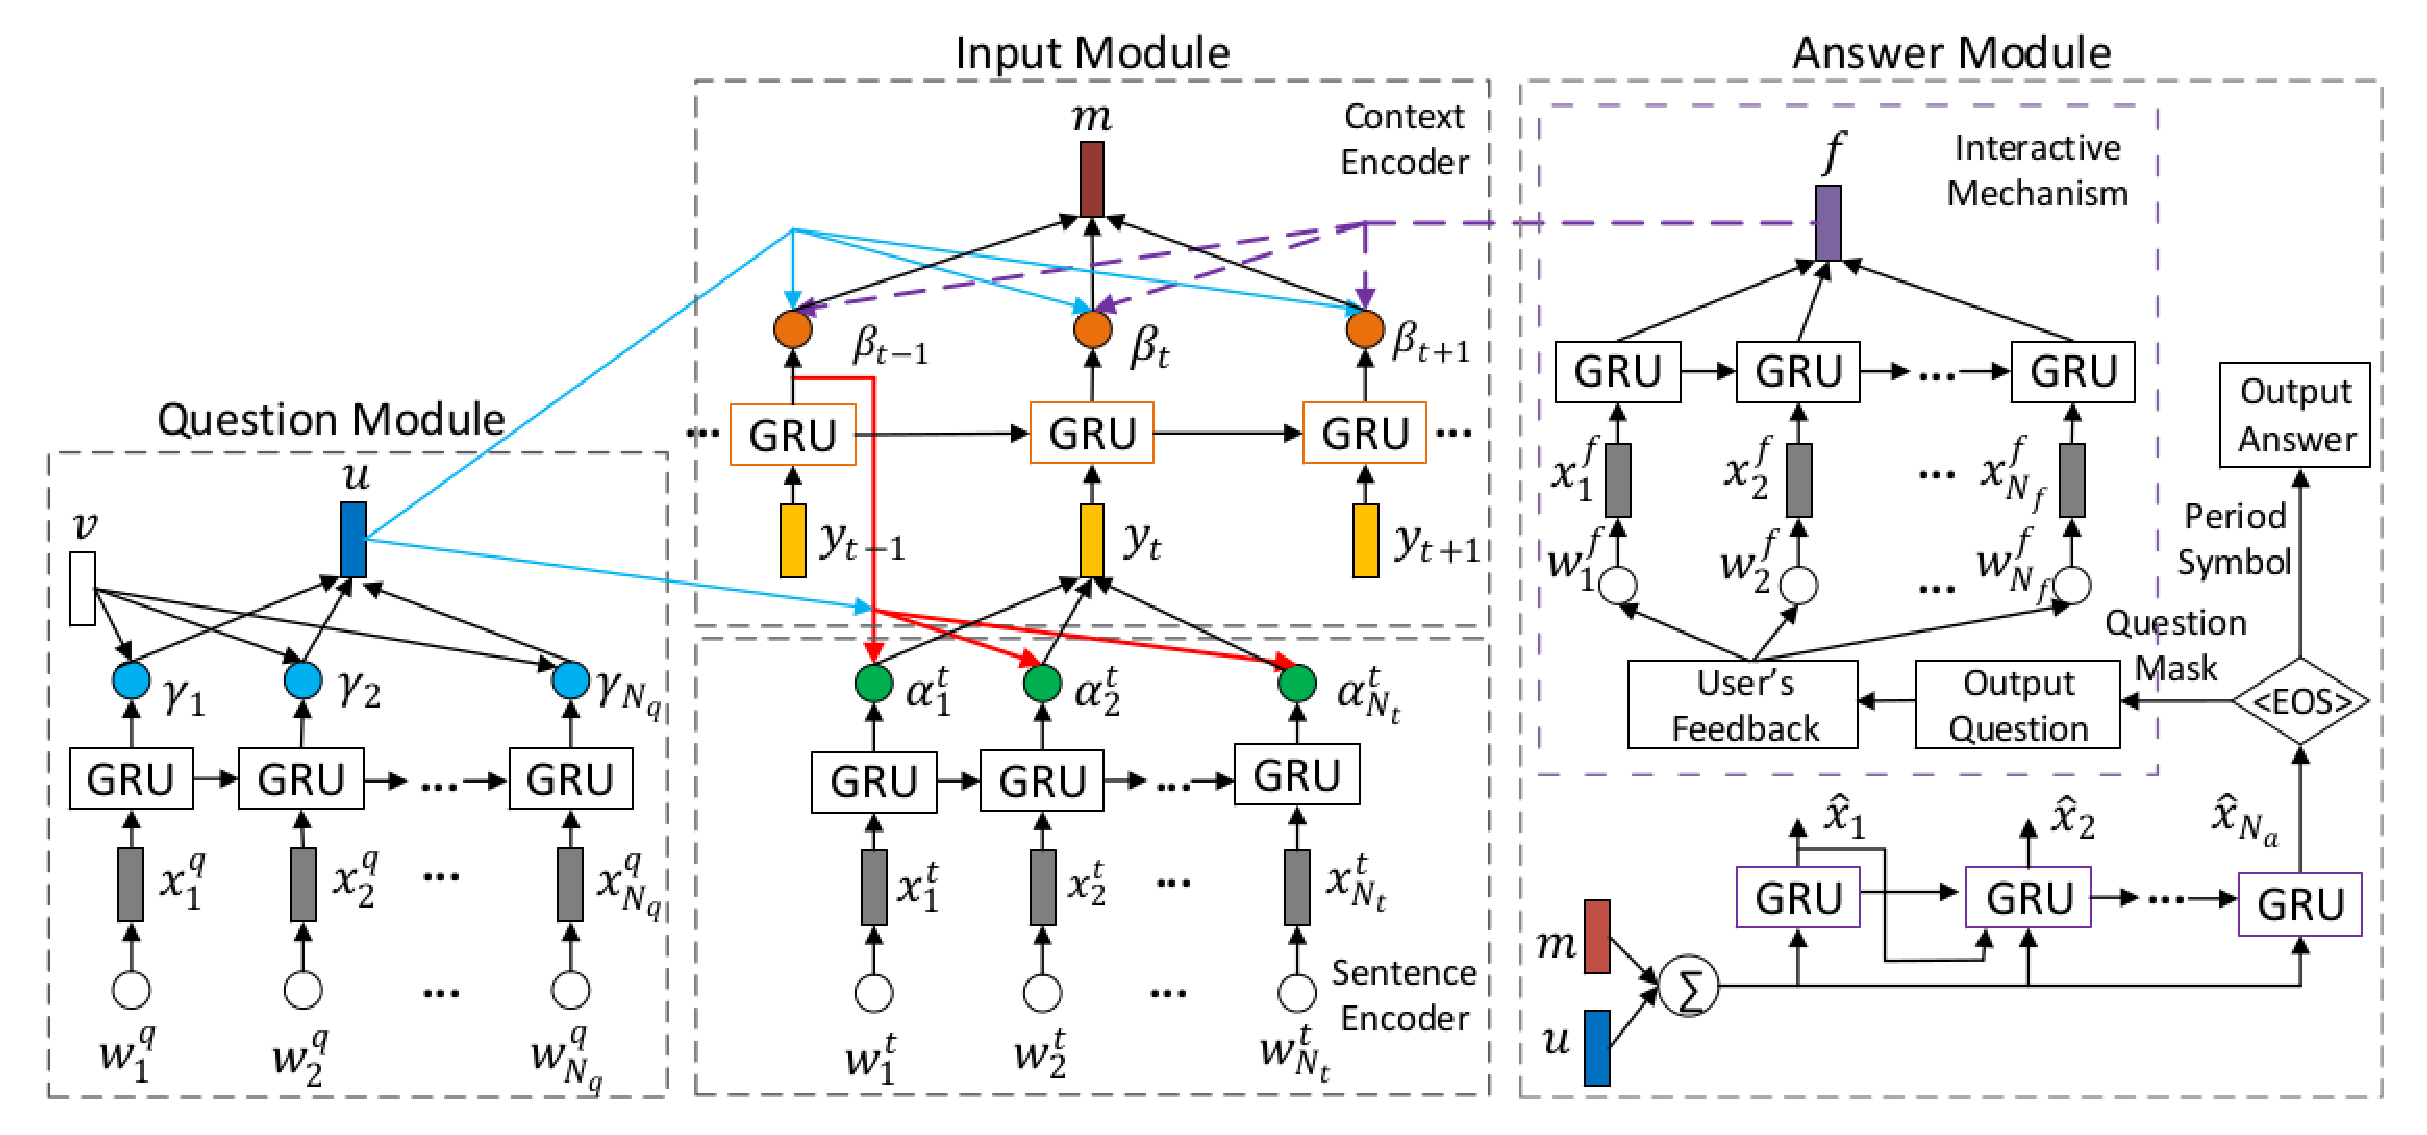
\includegraphics[height=5.25cm,width=0.7\textwidth]{Fig1.eps}
	\caption{}
	\vspace{-14pt}
\end{wrapfigure}
Question Answering is a discipline in Computer Science, specifically in the realm of natural language processing, that aims at automatically answering questions from user input. Current implementations of QA systems are based on statement-question-answer triplets \\ where each input sentence is mapped to an input representation space regarded as a memory component. The output representation is calculated by summarizing over input representations with different attention weights. This
single-layer memory is extended to multi-layer memory by reasoning the statements and the question with multiple hops \cite{paper}. This approach presents several limitations. The first problem is not determing the context of the word(s) in a sentence. Second is when the input-question pair fails to provide enough information regarding the question. An example of this is the triplet (\{The master bedroom is north of the kitchen. The guest bedroom is east of the office\}, What is the bedroom east of?, Unknown) \cite{paper}. The ambiguity of which bedroom leads to this failure. In contrast, the Context aware Attention Network (CAN) presented in this paper learns proper word contextual representation and interacts with the user if ambiguity is present in the answer processing phase. Figure 1 illustrates what goes on in the CAN implementation. To understand what is going on let us discuss in detail what happens at each step: 

\begin{figure}[!htb]
	\minipage{1\textwidth}
	\textbf{Question Module}
	\begin{enumerate}[wide, labelwidth=!, labelindent=0pt]
		\item Words $w_1^q, \dots, w_{N_q}^q$ are mapped to one-hot vectors $x_1^q, \dots, x_{N_q}^q$.
		\item Vectors $x_1^q, \dots, x_{N_q}^q$ are fed into GRUs that generate importance weights $\gamma_1, \dots, \gamma_{N_q}$ based on vocabulary $v$ and context.
		\item The question representation $u$ is then generated by a sum of $x_1^q, \dots, x_{N_q}^q$ weighted by $\gamma_1, \dots, \gamma_{N_q}$ and passed to the Input Module.
	\end{enumerate}
	\endminipage\hfill
\end{figure}

\newpage

\begin{figure}[!htb]
	\minipage{1\textwidth}
	\textbf{Input Module}
	\begin{enumerate}[wide, labelwidth=!, labelindent=0pt]
		\item For each input sentence $l_t$ each word $w_i$ is embedded into a word space $x_i^t$ through the shared learned embedding matrix, and a recurrent neural network is used to capture the context information from the words in the same sentence.
		\item GRUs compute each word annotation vector $h_1^t, \dots, h_{N_t}^t$ (this is a hidden state).
		\item Sentence representation $y_t$ is generated by aggregating $h_1^t, \dots, h_{N_t}^t$, computed with the same GRUs in the previous hidden state, with weights $\alpha_1^t, \dots, \alpha_{N_t}^t$.
		\item Weights $\beta_i$ are calculated in the GRUs.
		\item Context representation vector $m$ is calculated by summing over $y_1, \dots, y_t$ weighted by their corresponding $\beta_i$ weights. 
	\end{enumerate}
	\endminipage\hfill
\end{figure}

\begin{figure}[!htb]
	\minipage{1\textwidth}
	\textbf{Answer Module}
	\begin{enumerate}[wide, labelwidth=!, labelindent=0pt]
	\item Vectors $u$ and $m$ are summed together and passed to GRUs to compute predicted word vectors $\hat{x}_1, \dots, \hat{x}_{N_\alpha}$.
	\item If enough information is present for the answer, return output and terminate, else go to step 3.
	\item Ask the user a question to get more information; user responds with a sequence of words $w_1^f, \dots, w^f_{N_f}$ and mapped to vectors $x_1^f, \dots, x_{N_f}^f$.
	\item Corresponding annotation vectors $g_1^f, \dots, g_d^f$ and a representation $f$ is constructed via aggregation of annotation vectors.  
	\item Representation $f$ is then used to produce an answer based on the user's feedback.
	\end{enumerate}
	\endminipage\hfill
\end{figure}

Future work for the CAN implementation can include applications in commercial QA systems, such as Amazon echo or Google home. As we progress further, smart technology is becoming ever more so present in our homes and I feel that this will be the primary application of intelligent QA systems.

\vspace{0.25cm}
Three strengths of the paper I found were 
\begin{enumerate}
	\item The CAN QA system implements contextual awareness and user feedback during the answer module, allowing almost perfect responses to user input. 
	\item It is based upon previous work [2] making it an easy system to learn by those already involved in this field of research.
	\item The framework of the CAN QA system makes it easily applicable to commercial systems, such as the Amazon echo, due to it's reliance on user input for ambiguity rather than highest likely match.  
\end{enumerate}

\vspace{0.25cm}
Three weaknesses I found with the paper are 
\begin{enumerate}
	\item The additional computational complexity of the CAN QA system seems like it might add time to user's answers, making it inefficient for commercial products. The fact that the authors did not really talk over computational time complexity hints at this fact.
	\item User feedback for the answer module can actually confuse the CAN QA system if the feedback is incorrect since there does not seem to be any error checking at this stage.
	\item The framework of the CAN QA system does not seem to allow for parallelization making scalability hard for the future. 
\end{enumerate}

\vspace{0.25cm}
Questions for the presenter
\begin{enumerate}
	\item What happens if the user asks a question totally unrelated to the input that requires some prior knowledge from the user?
	\item What is the systems response to input with no logical sequence or context?
\end{enumerate}

\begin{thebibliography}{unsrt}
	\bibitem{paper}
	Huayu Li , Martin Renqiang Min , Yong Ge , Asim Kadav \emph{A Context-aware Attention Network for Interactive Question Answering}, KDD’17, August 13–17, 2017, Halifax, NS, Canada.
	\bibitem{complimentatry}
	Ankit Kumar, Ozan Irsoy, Peter Ondruska, Mohit Iyyer, James Bradbury, Ishaan
	Gulrajani, Victor Zhong, Romain Paulus, and Richard Socher. 2016. Ask Me
	Anything: Dynamic Memory Networks for Natural Language Processing. In
	ICML. 1378–1387.
\end{thebibliography}

\end{document}